\documentclass[14pt]{extarticle}
\usepackage[utf8]{inputenc}
\usepackage[T1]{fontenc}
\usepackage[spanish,es-lcroman]{babel}
\usepackage{amsmath}
\usepackage{amsthm}
\usepackage{physics}
\usepackage{tikz}
\usepackage{float}
\usepackage[autostyle,spanish=mexican]{csquotes}
\usepackage[per-mode=symbol]{siunitx}
\usepackage{gensymb}
\usepackage{multicol}
\usepackage{enumitem}
\usepackage[left=2.00cm, right=2.00cm, top=2.00cm, 
     bottom=2.00cm]{geometry}

%\renewcommand{\questionlabel}{\thequestion)}
\decimalpoint
\sisetup{bracket-numbers = false}

\title{\vspace*{-2cm} Práctica 6 - Ley de Ohm\\  Física III \vspace{-5ex}}
\date{}

\begin{document}
\maketitle

\section{Datos para la práctica.}

\begin{itemize}
\itemsep0em 
\item  \textbf{Práctica:} 6.
\item \textbf{Unidad:} Dos.
\item \textbf{Temática:} Electricidad.
\item \textbf{Nombre de la práctica:} Ley de Ohm.
\item \textbf{Número de sesiones que se requieren para la práctica:} Dos.
\item \textbf{Objetivo general: } Comprobar experimentalmente la relación entre la corriente eléctrica, el voltaje y la resistencia.
\item \textbf{Objetivos específicos: }
\begin{enumerate}
\item Operar el multímetro para realizar mediciones de corriente y voltaje directo, corriente y voltaje alterno y de resistencia eléctrica.
\end{enumerate}
\item \textbf{Hipótesis: } En un circuito eléctrico cerrado, el voltaje es directamente proporcional al producto de la corriente eléctrica y la resistencia. 
\end{itemize}

\section{Planteamiento del problema.} 

La resistencia de un material $(R)$ se define como la oposición a que fluya la carga eléctrica. Aunque la mayoría de los metales son buenos conductores de la electricidad, todos ofrecen cierta oposición a que el flujo de carga eléctrica pase a través de ellos. Esta resistencia eléctrica es un valor constante para gran número de materiales específicos, de tamaño, forma y temperatura conocidos. Y es independiente del voltaje aplicado y de la corriente que pasa a través de ellos.
\par
El primero en estudiar cuantitativamente los efectos de la resistencia para limitar el flujo de carga fue George Simon Ohm, en 1826. Él descubrió que, para una resistencia dada a una temperatura particular, la corriente es directamente proporcional al voltaje aplicado. Así como la rapidez de flujo de agua entre dos puntos depende de la diferencia de altura que hay entre ambos, la rapidez de flujo de la carga eléctrica entre dos puntos depende de la diferencia de potencial que existe entre ellos. Esta proporcionalidad se conoce, en general, como la ley de Ohm:
\textit{La corriente que circula por un conductor dado es directamente proporcional a la diferencia de potencial (voltaje) entre sus puntos extremos}.
\par
La expresión para la ley de Ohm es la siguiente:
\begin{align*}
V = I \, R
\end{align*}
La unidad de la resistencia es el Ohm $(\Omega)$.

\section{Marco teórico.}

\begin{enumerate}[label=\alph*)]
\item ¿Qué es la diferencia de potencial eléctrico?
\item Los materiales cuentan con la propiedad de resistividad eléctrica, ¿en qué consiste esta propiedad?
\item Revisa en un libro o sitio de física los valores de resistividad eléctrica de la porcelana, cobre, madera, plata, oro, y carbón, ordena los materiales de menor a mayor resistividad eléctrica. ¿Qué deducimos de la lista ordenada?
\end{enumerate}

\section{Material.}

\begin{enumerate}[label=\roman*)]
\begin{minipage}[t]{8cm}
\item 1 Multímetro.
\item 3 resistencias de distintos valores.
\item 1 pila AA.
\end{minipage}
\hspace{1cm}
\begin{minipage}[t]{4cm}
\item 1 pila AAA.
\item 1 pila 9 Volts.
\end{minipage}
\end{enumerate}


\section{Montaje experimental.}

\begin{enumerate}
\item Atiende las indicaciones del Profesor para el manejo cuidadoso del multímetro.
\item Coloca el dial del multímetro en la posición de \textbf{voltaje directo} 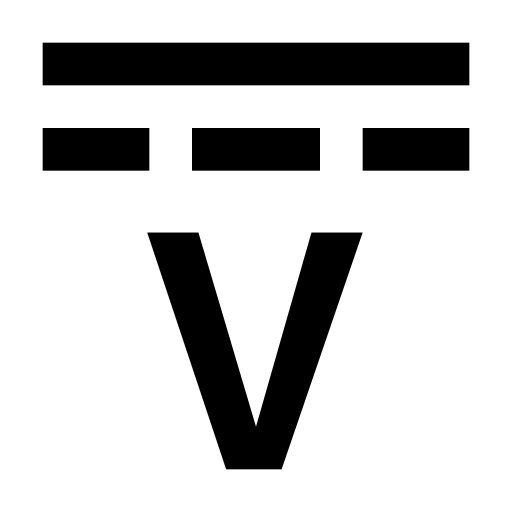
\includegraphics[scale=0.05]{Imagenes/voltage-dc.png}
\item Mide el voltaje de cada una de las pilas: AA, AAA y 9 V, anota los valores: \\
Pila AA: \rule{2cm}{0.1mm} \\
Pila AAA: \rule{2cm}{0.1mm} \\
Pila 9 V: \rule{2cm}{0.1mm}
\item Coloca el dial del multímetro en la posición de \textbf{voltaje alterno} 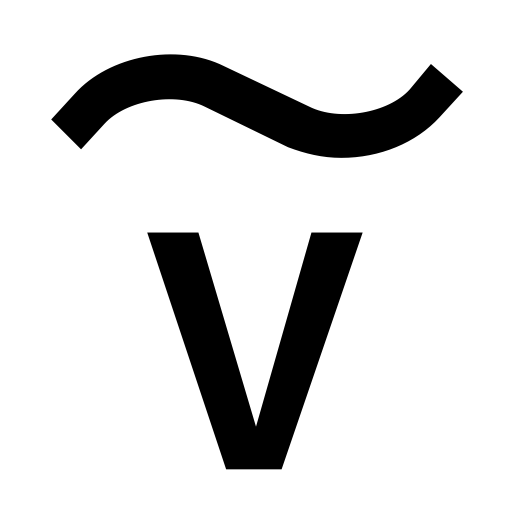
\includegraphics[scale=0.05]{Imagenes/voltage-ac.png}
\item Con las puntas en el multímetro, conecta las mismas en el contacto de la mesa de trabajo. Registra el valor que indica la pantalla: \rule{2cm}{0.1mm}
% \item Con el código de colores, identifica el valor de las resistencias y anótalo en la siguiente tabla (cada integrante del equipo deberá leer valor, no se permite que intercambien los datos, ya que se pedirá que lean el valor estando el Profesor presente):
\item Coloca el dial del multímetro en la posición de \textbf{resistencia} {\huge{$\Omega$}}
\item Mide el valor en la pantalla del multímetro y anótalo también en la siguiente tabla:
\begin{table}[H]
\centering
\begin{tabular}{| c | c |} \hline
Resistencia & Valor multímetro $(\Omega)$ \\ \hline
$R_{1}$ & \\ \hline
$R_{2}$ & \\ \hline
$R_{3}$ & \\ \hline
\end{tabular}
\end{table}
% \item Coloca el dial del multímetro en la posición de \textbf{corriente directa}.
% \item Establece un circuito en serie con la pila AA, el multímetro y la resistencia.
% \item Mide el valor de la corriente (en Amperes) que indica la carátula del aparato. Anota el valor en la siguiente tabla.
% \begin{table}[H]
% \centering
% \begin{tabular}{| c | c | } \hline
% Resistencia & Corriente $(\si{\ampere})$ \\ \hline
% $R_{1}$ & \\ \hline
% $R_{2}$ & \\ \hline
% $R_{3}$ & \\ \hline
% \end{tabular}
% \end{table}
\end{enumerate}

\end{document}